% -----------------------------------------------------------------------------
%                                 Research Directions
% -----------------------------------------------------------------------------

\newpage                                          \chapter{Research Directions}

\begin{figure}[htbp2]
  \begin{minipage}[b]{.45\linewidth}
    \centering
  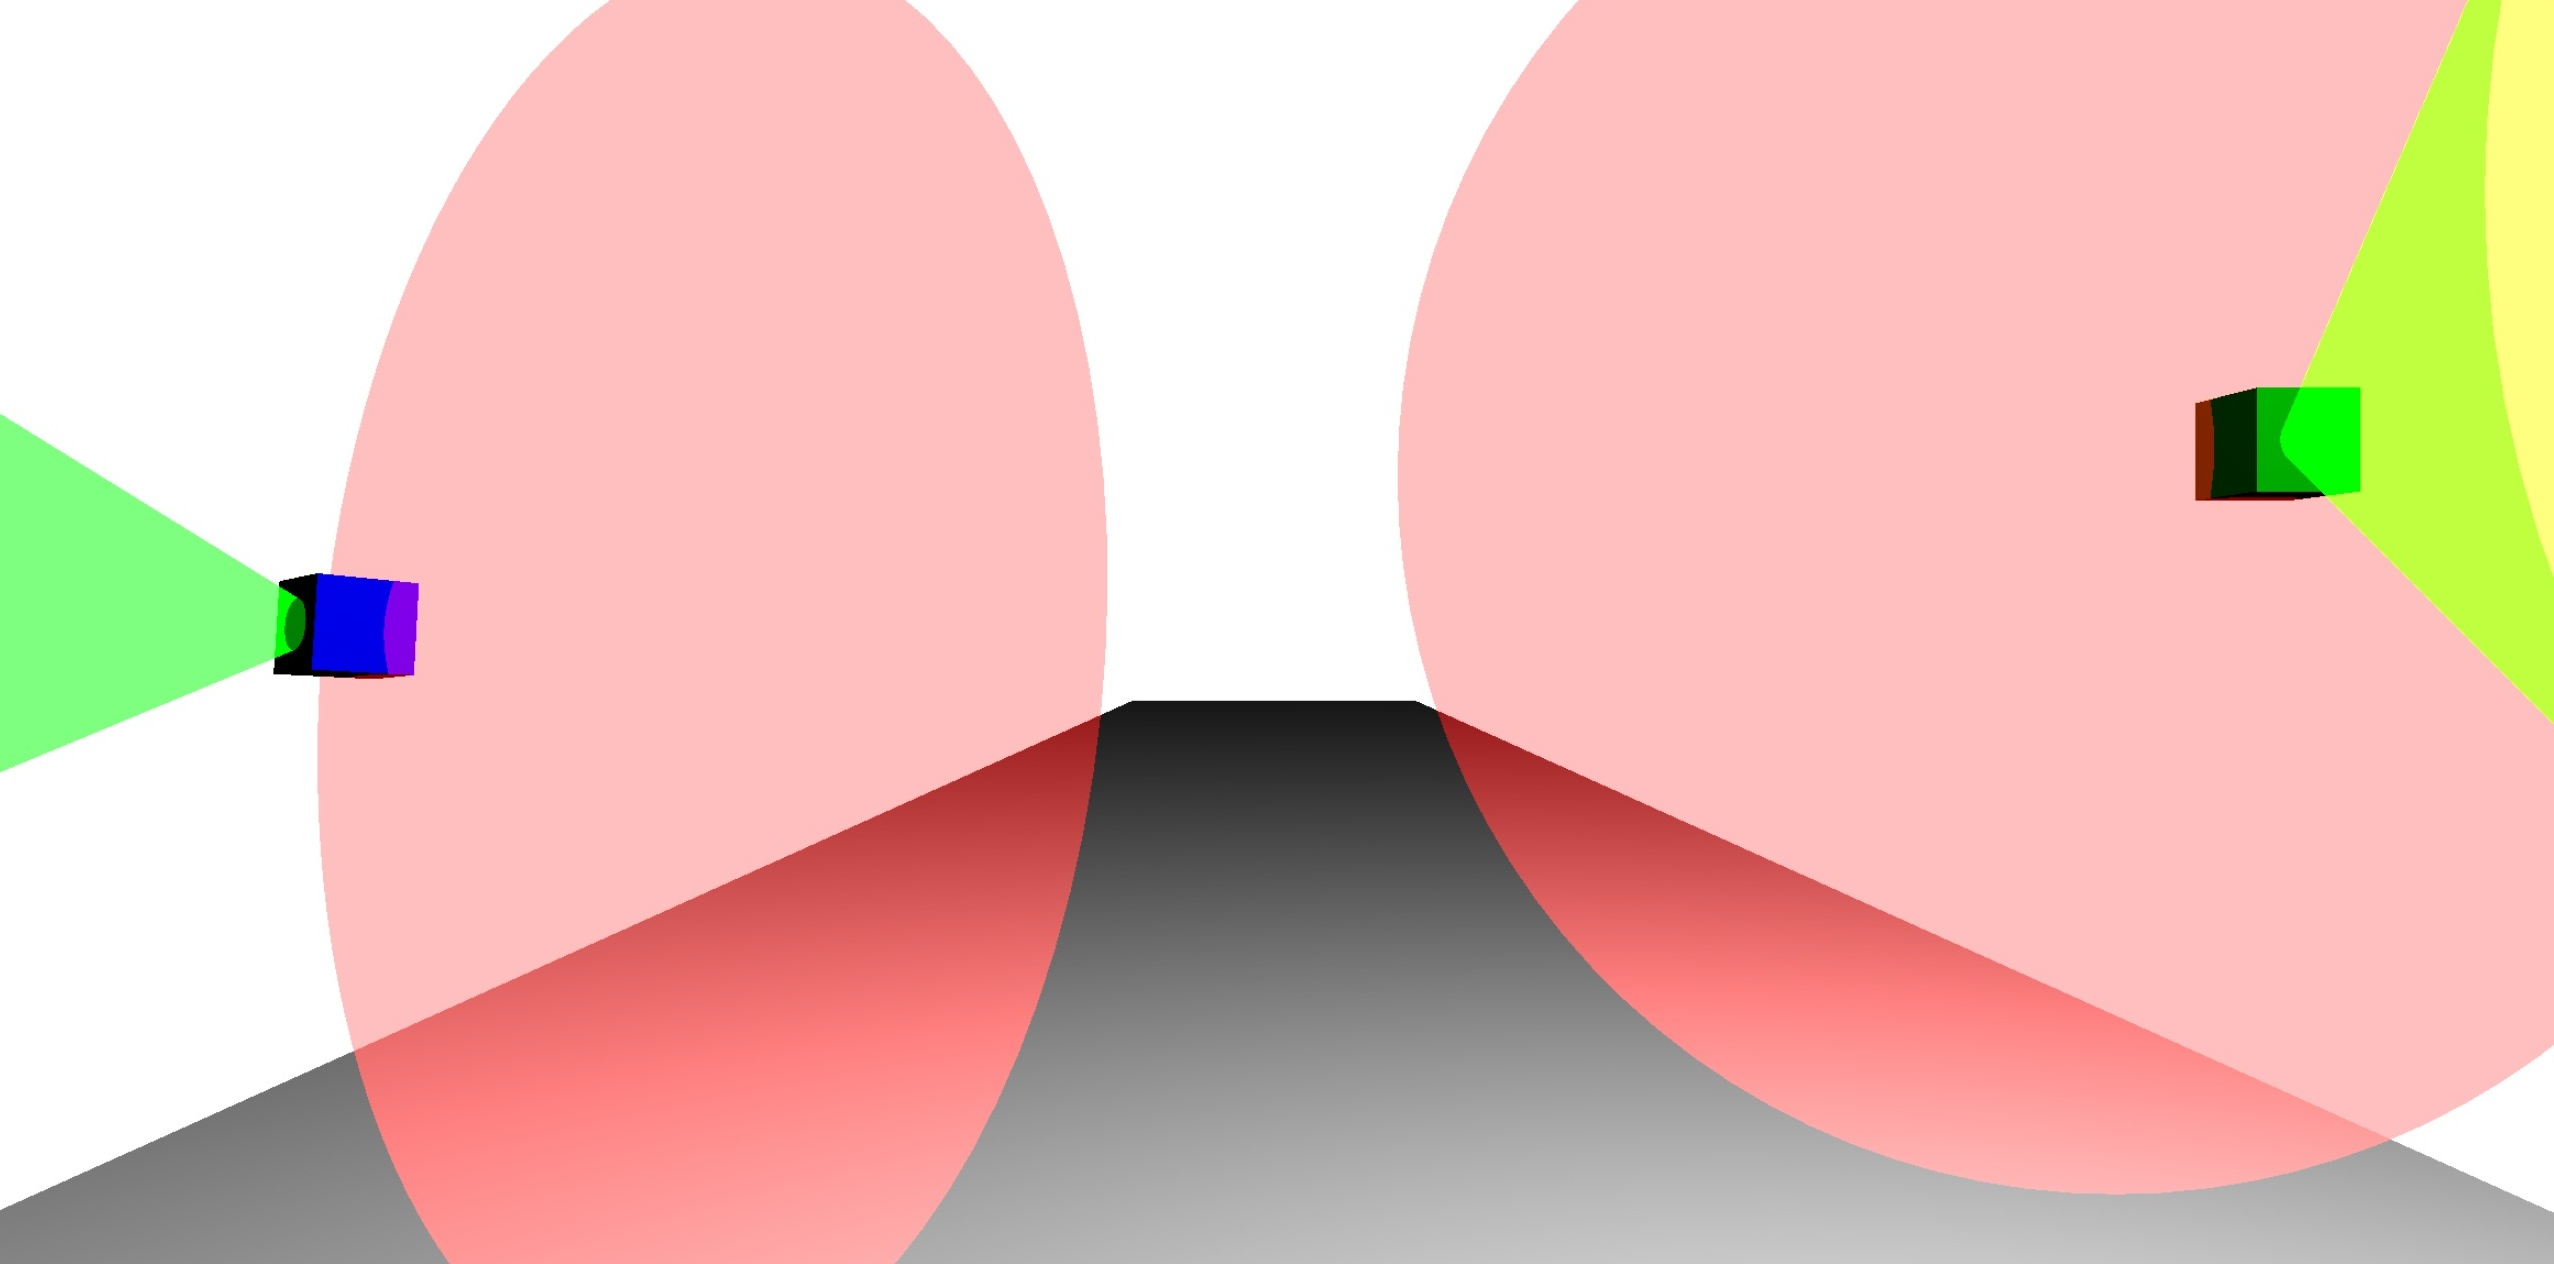
\includegraphics[width=1\linewidth]{images/irys_screenshot.jpg}
    \caption{   \small
 Sample rendition of sound images in 3D space}
    \label{fig:irys}
  \end{minipage}
  \hspace{0.5cm}
  \begin{minipage}[b]{0.45\linewidth}
    \centering
  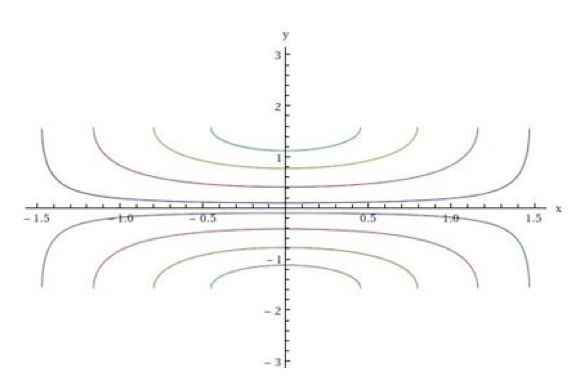
\includegraphics[width=1\linewidth]{images/irys_pathways.jpg}
    \caption{  \small Sample sound paths tested}
    \label{fig:irys_paths}
  \end{minipage}
\end{figure}

This project explores previous work which have utilized 3D audio.  This thesis
hopes to develop a road map for future work that might outline future research's
path to understanding the full potential that a binaural interface might
provide.  As an interface places sound images around the user, new methods of
information  portrayal are provided to users as the interface's 3D sound
environment allows for users to interact with technology when visual attention
is either not  available or not desired.

Before considering the state of prior art, it is important to clarify the
technical concepts of interest and which ones we plan to avoid. For example,
conventional binaural or transaural audio systems work well if the listener is
stationary at the position (usually along the perpendicular bisector of the two
points of sound) as  graphically represented by rendition~\ref{fig:irys}.
However, once the listener moves away from the sweet spot, system performance
degrades rapidly. There has been previous work in addressing the physics of this
problem ~\cite{song2010personal} but, because headphones alleviate these
problems (as the user's location does not change relative to a sweet spot), we
will simplify our system and not explore those types of technical questions.

For this project, we will not concern ourselves with the case that the user is
moving independent of the audio source and assume that the user is either in a
stationary environment or has headphones to remove the need for external
monitoring and real time updating of the audio transformations.

This section presents possible points of exploration that can be used to
understand how 3D audio algorithms can be used to create new types of interfaces
and the  implications they have on usability. By building interfaces that draw
audio images  as depicted by the virtual rendition found in
figure~\ref{fig:irys}, binaural audio may be used to provide a more efficient
interface when vision is not available.  An environment that allows sound images
to be placed arbitrarily around the user, content that is depicted audibly can
be manipulated to drive a number of key  metrics. In this section, we enumerate
the direction of future work and the  proposed aspects of exploration.

%----------------------------------------------------------------------------%
\subsection{                  Notifications                                  }

The essence of any event or update to user data is condensed into a
notification.  Current research has explored how notification systems attempt to
deliver current, important information to computer screens.  Previous works have
also explored the costs, benefits, and optimal displays of these notifications
from psychological perspectives that overlap with our ability to handle
interruptions and distractions~\cite{McCrickard2003509,
cutrell2001notification}. In this regard, any exploration of a binaural interface
should empirically test the value of choosing different types of notifications
and the presentation of the notifications to the user.


\subsection{                  Current Results and Frameworks                  }

Currently, a prototype of a web enabled binaural audio system has been developed.
The prototype is a personal 3D audio system that can be used to draw sound images
around a user. The virtual environment created allows the user to interact with 
the space and sound, moving independently of the sound sources. The system can 
then recalculate the necessary HRTFs relative to the user's updated position in
real time. The goal for this prototype was to create a development environment 
that allows a developer to use sound images to explore the interfaces efficacy 
in presenting content to a user without a visual display. The existing work
has explored four physical interfaces : native desktop applications, Android
handhelds, iOS handhelds, and the web. Each medium provides different drawbacks
and benefits for the interface being built. Most importantly, the prototype 
demonstrates the availability of the necessary computing power in mobile 
devices to create 3D audio environments and the ability of the web to present 
that content.\\

\textbf{OpenAL} is a cross-platform open sourced library that provides
efficient rendering of multichannel three-dimensional positional audio.  It has
implementations on most native  application frameworks, and at the onset of the
project, seemed to provide a silver bullet for much of the interface across
multiple devices.  During the implementation cycle of this project, I found
that OpenAL provided exciting abstractions, but distance was only provided by
volume amplitude attenuation and not properly calculated with a delay.

Creating a native desktop, iOS and android application using OpenAL was quick,
but upon evaluation by  human subjects, it became apparent that the framework
was too limiting.  By using volume to place the sound, the user was left with
jarring edge conditions as the sound image crossed planes of reference.
Figure 3 represents pathways tested on users, where each line
represents a sound traversal pattern relative to the user centered at the
origin. Because OpenAL uses volume based attenuation and not delays in sound
queuing, items were perceived to be traveling along a single flattened left-to-
right (x-axis) plane.

Despite the flattening perception of the library, it was a great tool to test
some of the concepts on both mobile and desktop environments to initially
understand if such a framework was feasible and useful.  With OpenAL, a
framework is provided that allows for audio streams to be created and played in
real-time (this is contrary to what can currently be done on the web, as HTML
requires that the audio to be played already exist).

\textbf{HTML5} For the web, we were able to utilize a new audio tag introduced
by the web standard community.  The new HTML5 audio tag allowed us to modify the
JavaScript on web pages to generate the necessary transforms and delays to
place the sound in a 3D environment.  Using the library Three.js we were also
able to create the necessary callback scripts to perform the transformations as
well.

The framework we present here, allows an individual to occupy a space and
interact with the surroundings.  The browser is able to perform the necessary
transformations and displace the audio around the user in real time. It is the
platform of choice as it is available across all devices and currently only
relies on the availability of an HTML5 compliant browser and a device that
can produce stereo sound.
